% To je predloga za poročilo projekta pripredmetu Osnove verjetnosti in
% statistike.
% Originalen avtor predloge je Blaž Zupan.
% Za potrebe OVS je prilagodil Robert Cvitkovič
% To predlogo lahko spremeniš v PDF dokument s pomočjo programa
% pdflatex, ki je del standardne instalacije LaTeX programov.

\documentclass[a4paper,11pt]{article}
\usepackage[utf8]{inputenc}
\usepackage{amsmath, amssymb, amsthm, amsfonts, mathtools}
\usepackage{a4wide}
\usepackage[slovene]{babel}
\usepackage{graphicx}
\usepackage{url}
\usepackage{float}
\usepackage[pdftex,pdfpagelabels,bookmarks,hyperindex,hyperfigures]{hyperref}

% \usepackage{tikz}
% \usepackage{pgflibraryshapes}

\usepackage[footnotesize,labelfont=bf,labelsep=period]{caption}
\usepackage{enumerate}


% \usepackage{hyperref}
\hypersetup{
pdffitwindow=true,              % window fit to page when opened
pdftitle={The Sylvester graph and Moore graphs},       % title
pdfauthor={Janko in Metka},                % author
pdfnewwindow=true,              % links in new window
colorlinks=true,                % false: boxed links; true: colored links
linkcolor=blue,                 % color of internal links
citecolor=blue,                 % color of links to bibliography
filecolor=blue,                 % color of file links
urlcolor=cyan                   % color of external links
}



\newcommand{\doi}[1]{\href{http://dx.doi.org/#1}{\texttt{doi:#1}}}
\newcommand{\arxiv}[1]{\href{http://arxiv.org/abs/#1}{\texttt{arXiv:#1}}}




\title{Naslov seminarske naloge}
\author{Ime Priimek} % (vpisna številka)}
\date{\today}

\begin{document}

\maketitle

\section{Uvod}

% V tem razdelku, 
% ki naj bo kratek in naj obsega en odstavek z do 150 besed, 
% na kratko opišeš, kaj je bil cilj naloge.

Uvod naj bi imel približno naslednjo strukturo:
\begin{itemize}
\item vaba/motivacija (zakaj je tema zanimiva - najbolje skozi
      kakšen provokativen primer)
\item problem/cilj (le ta mora biti vedno jasno opisan)
\item podobne raziskave (ki postavijo Tvoje delo v kontekst)
\item kratka organizacija po poglavijih/razdelkih 
\end{itemize}
%
Imena poglavij 
\begin{enumerate}
\item Uvod
\item Podatki
\item Izračuni in rezultati
\item Zaključek
\item Literatura (no tu ne sme pisati ``References'')
\end{enumerate}
pa seveda priredite glede na svojo vsebino.


\section{Podatki}

Če je naloga zasnovana tako, da vključuje analizo izbranih podatkov, v
tem razdelku opišeš, kakšni so ti podatki in navedeš nekaj osnovnih
statističnih lastnosti teh podatkov. Slednje vključujejo velikost
podatkov (na primer število primerov, število in vrsto atributov), delež
manjkajočih podatkov, opis in porazdelitev vrednosti ciljnih
spremenljivk, in podobno. Če si podatke pridobil sam, tu opišeš, na
kakšen način, kje in kako.

\section{Izracuni in rezultati}

Rezultate lahko prikažeš tudi v tabeli~\ref{tab1} ali sliki~\ref{slika1}. 
Vse slike in tabele, ki jih vključiš v poročilo, morajo biti navedene v 
besedilu oziroma se moraš na njih sklicati.

\begin{figure}[htbp]
\begin{center}
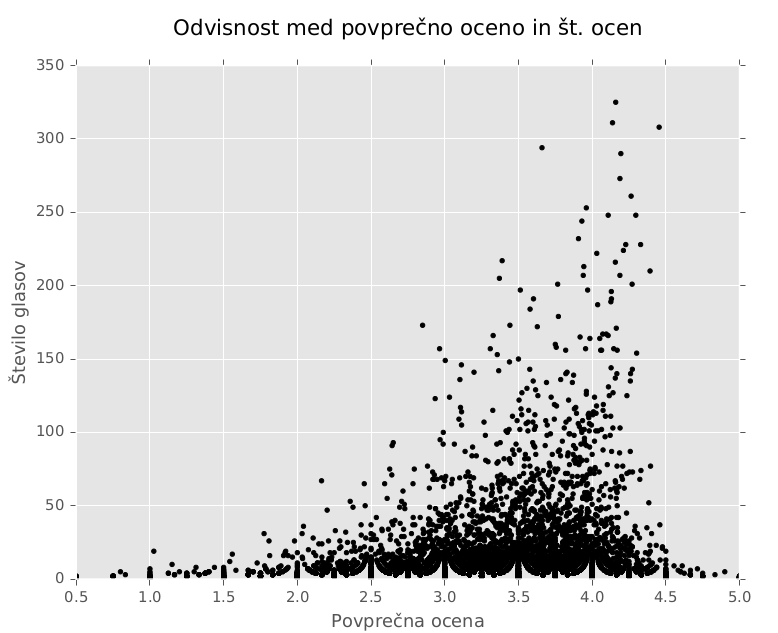
\includegraphics[scale=0.5]{slika-primer.png}
\caption{Vsako sliko opremi s podnapisom, ki pove, kaj slika prikazuje.}
\label{slika1}
\end{center}
\end{figure}

Odstavke pri pisanju poročila v LaTeX-u ločiš tako, da pred novim
odstavkom pustiš prazno vrstico.
\begin{table}[htbp]
\caption{Atributi in njihove zaloge vrednosti.}
\label{tab1}
\begin{center}
\begin{tabular}{llp{3cm}}
\hline
ime spremenljivke & definicijsko območje & opis \\
\hline
cena & [0, 500] & cena izdelka v EUR\\
teža & [1, 1000] & teža izdelka v dag \\
kakovost & [slaba|srednja|dobra] & kakovost izdelka \\
\hline
\end{tabular}
\end{center}
\end{table}

LaTeX ti omogoča tudi zelo enostaven in lep izris enačb tako znotraj vrstice
($\alpha = \beta + 90^{\circ}$), kot med vrsticami.

$$\sigma^2 = \frac{(\bar{x} - x_i)^2}{N}$$

\section{Zakljucek}

V tem poglavju na kratko povzameš rezultate in vso ostalo znanje, ki si ga pridobil
s tem projektom.

\section{Literatura}

Literatura bi mogla vsebovati vsaj eno knjigo (in ne samo našo
skripto - sploh pa nikjer ne piše, da gre za skripto, A. Jurišić bo
dovolj - polna imena so odveč), a še nekaj člankov (če si me vzel
resno glede konteksta - saj verjetno ne delaš prvi tovrstno raziskavo).

\begin{footnotesize}
\begin{thebibliography}{10}
\bibitem{g93}
C.~D. Godsil.
\newblock {\em Algebraic combinatorics}.
\newblock Chapman and Hall Mathematics Series. Chap\-man \& Hall, New York,
1993.

\bibitem{gr01}
C.~D. Godsil and G.~Royle.
\newblock {\em Algebraic graph theory}, volume 207 of {\em Graduate Texts in
Mathematics}.
\newblock Springer-Verlag, New York, 2001.


\bibitem{j95}
A.~Jurišić.
\newblock {\em Antipodal covers}.
\newblock PhD thesis, University of Waterloo (Canada), 1995.

\bibitem{jv12}
A.~Jurišić and J.~Vidali.
\newblock Extremal $1$-codes in distance-regular graphs of dia\-meter~$3$.
\newblock {\em Des. Codes Cryptogr.}, 65(1--2):29--47, 2012.
\newblock \doi{10.1007/s10623-012-9651-0}.

\end{thebibliography}
\end{footnotesize}

\end{document}
